\subsection{The Proof That Broke Their Brains}

\begin{enumerate}
\item Suppose that \( \sqrt{2} \) can be written as a fraction:

   \[
   \sqrt{2} = \frac{p}{q}
   \]

   where \( p \) and \( q \) have \textbf{no common factors}.

\item Squaring both sides:

   \[
   2 = \frac{p^2}{q^2}
   \]

\item Multiplying both sides by \( q^2 \):

   \[
   2q^2 = p^2
   \]

   which means \( p^2 \) is \textbf{even}, so \( p \) itself must be even. That means we can write \( p = 2k \) for some integer \( k \).

\item Substituting:

   \[
   2q^2 = (2k)^2 = 4k^2
   \]

   Dividing both sides by 2:

   \[
   q^2 = 2k^2
   \]

   which means \( q^2 \) is also even, so \( q \) must also be even.

\item \textbf{But if both \( p \) and \( q \) are even, that means they share a common factor of 2}, contradicting our original assumption.

\item \textbf{Oops. That means our assumption was wrong.} Which means:

   \[
   \sqrt{2} \text{ is NOT a fraction.}
   \]

\end{enumerate}   
   

This was bad news for the Pythagoreans. Their entire worldview was built on the idea that numbers were clean, perfect, and rational. And now, here was a number that refused to fit into their system.

\begin{figure}[H]
\centering
\begin{tikzpicture}[every node/.style={font=\footnotesize}]

% Panel 1 — Philosopher starting the proof confidently
\comicpanel{0}{4}
  {Hippasus}
  {}
  {\textbf{Philosopher:} Suppose \(\sqrt{2} = \frac{p}{q}\), where \(p\) and \(q\) have no common factors. Easy. Let’s go.}
  {(0,-0.5)}

% Panel 2 — Philosopher mid-proof, raising eyebrows
\comicpanel{6.5}{4}
  {Hippasus}
  {}
  {\textbf{Philosopher:} So... \(2q^2 = p^2\).  
That means \(p\) is even.  
Let’s write \(p = 2k\)...}
  {(0,-0.5)}

% Panel 3 — Philosopher looking increasingly worried
\comicpanel{0}{0}
  {Hippasus}
  {}
  {\textbf{Philosopher:} Wait.  
Then \(q\) is also even?  
But... that means they share a factor of 2.  
But they weren’t supposed to!}
  {(0,0.8)}

% Panel 4 — Philosopher staring into the void
\comicpanel{6.5}{0}
  {Hippasus}
  {}
  {\textbf{Philosopher:} \(\sqrt{2}\) isn’t rational.  
Numbers are chaos.  
I’m going outside to scream.}
  {(0,0.8)}

\end{tikzpicture}
\caption{Discovering that \(\sqrt{2}\) is irrational: a proof so elegant it broke ancient brains.}
\end{figure}